\documentclass{article}

\usepackage{fancyhdr}
\usepackage{extramarks}
\usepackage{amsmath}
\usepackage{amsthm}
\usepackage{amsfonts}
\usepackage{tikz}
\usepackage[plain]{algorithm}
\usepackage{algpseudocode}
\usepackage{listings}
\usepackage{minted}
\usepackage[utf8]{inputenc}
\usepackage[english]{babel}
\usetikzlibrary{automata,positioning}
\usepackage{graphicx}
%
% Basic Document Settings
%


\topmargin=-0.45in
\evensidemargin=0in
\oddsidemargin=0in
\textwidth=6.5in
\textheight=9.0in
\headsep=0.25in

\linespread{1.1}

\pagestyle{fancy}
\lhead{\hmwkClass\ (\hmwkClassInstructor): \hmwkTitle}
\chead{\hspace{4.8in}\hmwkAuthorName}
\rhead{\firstxmark}
\lfoot{\lastxmark}
\cfoot{\thepage}

\renewcommand\headrulewidth{0.4pt}
\renewcommand\footrulewidth{0.4pt}

\setlength\parindent{0pt}

%
% Create Problem Sections
%

\newcommand{\enterProblemHeader}[1]{
    \nobreak\extramarks{}{Problem \arabic{#1} continued on next page\ldots}\nobreak{}
    \nobreak\extramarks{Problem \arabic{#1} (continued)}{Problem \arabic{#1} continued on next page\ldots}\nobreak{}
}

\newcommand{\exitProblemHeader}[1]{
    \nobreak\extramarks{Problem \arabic{#1} (continued)}{Problem \arabic{#1} continued on next page\ldots}\nobreak{}
    \stepcounter{#1}
    \nobreak\extramarks{Problem \arabic{#1}}{}\nobreak{}
}

\setcounter{secnumdepth}{0}
\newcounter{partCounter}


%
% Homework Problem Environment
%
% This environment takes an optional argument. When given, it will adjust the
% problem counter. This is useful for when the problems given for your
% assignment aren't sequential. See the last 3 problems of this template for an
% example.
%


%
% Homework Details
%   - Title
%   - Due date
%   - Class
%   - Section/Time
%   - Instructor
%   - Author
%

\newcommand{\hmwkTitle}{Homework 3}
\newcommand{\hmwkDueDate}{Tuesday, Feb 29, 2016}
\newcommand{\hmwkClass}{DS-GA 1003}
\newcommand{\hmwkClassInstructor}{Professor David Ronsenberg}
\newcommand{\hmwkAuthorName}{Yuhao Zhao}
\newcommand{\hmwknetid}{Yz3085}
\newcommand{\hmwksubtitle}{SVM and Sentiment Analysis}
\newcommand{\gihub}{See complete code 00at: \textit{git@github.com:cryanzpj/1003.git}}
%
% Title Page
%

\title{
    \vspace{2in}
    \textmd{\textbf{\hmwkClass:\ \hmwkTitle \\ \hmwksubtitle }}\\
    \vspace{1in}
    \normalsize\vspace{0.1in}\small{Due\ on\ \hmwkDueDate}\\
    \vspace{0.1in}\large{\textit{\hmwkClassInstructor}}\\
    \vspace{3in}
    \author{\textbf{\hmwkAuthorName} \\ \textbf{\hmwknetid }\\ }
    \vspace{0.2in}
    \gihub
}



\date{}

\renewcommand{\part}[1]{\textbf{\large Part \Alph{partCounter}}\stepcounter{partCounter}\\}

%
% Various Helper Commands
%

% Useful for algorithms
\newcommand{\alg}[1]{\textsc{\bfseries \footnotesize #1}}

% For derivatives
\newcommand{\deriv}[1]{\frac{\mathrm{d}}{\mathrm{d}x} (#1)}

% For partial derivatives
\newcommand{\pderiv}[2]{\frac{\partial}{\partial #1} (#2)}

% Integral dx
\newcommand{\dx}{\mathrm{d}x}

% Alias for the Solution section header
\newcommand{\solution}{\textbf{\large Solution}}

% Probability commands: Expectation, Variance, Covariance, Bias
\newcommand{\E}{\mathrm{E}}
\newcommand{\Var}{\mathrm{Var}}
\newcommand{\Cov}{\mathrm{Cov}}
\newcommand{\Bias}{\mathrm{Bias}}


\newenvironment{problem}[2][$\bullet$]{\begin{trivlist}\large
		\item[\hskip \labelsep {\bfseries #1}\hskip \labelsep {\bfseries #2.}]}  {\end{trivlist}}

\newenvironment{sub}[2][$-$]{\begin{trivlist}
		\item[\hskip \labelsep {\bfseries #1}\hskip \labelsep {\bfseries #2.}]}  {\end{trivlist}}
\newenvironment{lemma}[2][Lemma]{\begin{trivlist}
		\item[\hskip \labelsep {\bfseries #1}\hskip \labelsep {\bfseries #2.}]}{\end{trivlist}}
\newenvironment{exercise}[2][Exercise]{\begin{trivlist}
		\item[\hskip \labelsep {\bfseries #1}\hskip \labelsep {\bfseries #2.}]}{\end{trivlist}}

\newenvironment{question}[2][Question]{\begin{trivlist}
		\item[\hskip \labelsep {\bfseries #1}\hskip \labelsep {\bfseries #2.}]}{\end{trivlist}}
\newenvironment{corollary}[2][Corollary]{\begin{trivlist}
		\item[\hskip \labelsep {\bfseries #1}\hskip \labelsep {\bfseries #2.}]}{\end{trivlist}}

\begin{document}

\maketitle

\pagebreak

\section{2. Calculating  Subgradients}

\begin{problem}{2.1 Subgradients for pointwise maximum of functions}
\end{problem}
Since $f = \max_{i=1,\ldots,,m}f_{i}(x)$. and $f_i $ is convex\\
for $\forall x,y,c$$$f(cy+(1-c)x) = \max_{i=1,\ldots,,m}f_{i}(cy+(1-c)x) \leq \max_{i=1,\ldots,,m} cf_i(y) + (1-c)f_i(x)\\ = cf(y) + (1-c)f(x)$$
Therefore, f is convex.  For any k that $f_k(x) = f(x)$ and $g \in \partial f_k(x) $
$$f_k(z) \geq f_k(x) + g^T (z-x)$$ Therefore, $$f(z) \geq f(x) + g^T(z-x)$$
This means $g \in \partial f(x)$

\begin{problem}{2.2 Subgradient of hinge loss for linear prediction}
\end{problem}
$$J(w) = \max \{0,1-yw^Tx\}$$
A subgradient of J is:\\
$$\begin{cases}
0 \quad , 1 -yw^Tx <0\\
-yx, otherwise
\end{cases}$$

\section{3. Perceptron}
\begin{sub}{3.1}
\end{sub}
If the data D are linearly separable, $\forall y_i = 1, \hat{y_i}= w^Tx_i <0 $ and $\forall y_i =-1, \hat{y_i} = w^Tx_i >0$ \\
This means $$\forall y_i, -y_i\hat{y_i} <0, l(\hat{y_i},y_i) = max\{0,-\hat{y_i}y_i\} = 0$$
the average perceptron loss on D is therefore 0. 

\begin{sub}{3.2}
\end{sub}
If we run SGD to minimize the empirical risk, the perceptron loss is  $ l(\hat{y_i},y_i) = max\{0,-y_iw^Tx_i\}$\\
A subgradient is $$\begin{cases}
0 \quad , -y_iw^Tx_i \leq 0\\
-y_ix_i, otherwise
\end{cases}$$
If we set step size = 1, we update w by:
$$w_{i+1} = \begin{cases}
w_i \quad , -y_iw_i^Tx_i \leq 0\\
w_i+y_ix_i, otherwise
\end{cases}$$
This is exactly the Perceptron Algorithm. 
\pagebreak


\begin{sub}{3.3}
\end{sub}
From the Perceptron Algorithm, in each step we update $w_i$ by adding $y_ix_i$ or 0 to $w_i$. \\Therefore, our output is actually $w_n = \sum \alpha_i x_i$\\
For $x_i$ that is a support vector, it satisfies that $-y_iw_i^Tx_i >0$, which $w_i$ is the weight vector at the i-th iteration. 


\section{4. The Data}
\begin{minted}{python}
def shuffle_data():
'''
pos_path is where you save positive review data.
neg_path is where you save negative review data.
return: shuffled data
'''
	pos_path = "/Users/cryan/Desktop/1003/github/as3/data/neg"
	neg_path = "/Users/cryan/Desktop/1003/github/as3/data/pos"
	
	pos_review = folder_list(pos_path,1)
	neg_review = folder_list(neg_path,-1)
	
	review = pos_review + neg_review
	random.shuffle(review)
return np.array(review)

data = np.array(shuffle_data())
data_train = data[:1500]
data_test = data[1500:]

np.save("X_train", map(lambda x: x[:-1],data_train))
np.save("X_test", map(lambda x: x[:-1],data_test))
np.save('Y_train', map(lambda x: x[-1],data_train))
np.save('Y_test', map(lambda x: x[-1],data_test))

\end{minted}

\section{5. Sparse Representation}

\begin{minted}{python}
def tokenlizer(text):
'''
converts a list of words into bag-of-words

Args:
text: a list of words

Returns: a dictionary/ hash table of text
'''
	res = Counter()
	for i in text:
		res[i] +=1
return res
\end{minted}

\pagebreak

\section{6. Support Vector Machine via Pegasos}

\begin{problem}{6.1}
\end{problem}
Since the objective function is :
$$L = \frac{\lambda}{2} ||w||^2 + \frac{1}{m} \sum max\{0,1-y_iw^Tx_i\}$$
With SGD, in each step, we are updating w w.r.t $\frac{\lambda}{2} ||w||^2 + max\{0,1-y_iw^Tx_i\}$\\
This objective function is convex, one subgradient is :
$$\begin{cases}
\lambda w \quad ,1 -y_iw^Tx_i \leq 0\\
\lambda w-y_ix_i , otherwise
\end{cases}$$
Then the corresponding update, if we choose $\eta_t = \frac{1}{\lambda t} $is :
$$w_{i+1} = \begin{cases}
 w_{i} -\lambda \eta_i w_i = (1 - \eta_i \lambda)w_i \quad ,1 -y_iw^Tx_i \leq 0\\
w_i - \eta_i ( \lambda w_i-y_ix_i ) = (1- \eta_i\lambda)w_i + \eta_iy_ix_i, otherwise
\end{cases}$$
This update is identical to the pseudocode. \\

\begin{problem}{6.2}
\end{problem}
\begin{minted}{python}
def pegasos_svm_sgd(X,y,lambda_ = 10,n_ite = 1,print_time = False):
'''
pegasos svm with pure sgd approach

Args:
X: Train data
y: Train lable
lambda_: regulization
n_ite: max iterations
print_time: whether count the operation time

Returns: sparse representaion of the weight

'''
X = np.array(map(lambda a: tokenlizer(a) , X),dtype = object)
num_instances = X.shape[0]
t = 0.0
n = 0
w = Counter()
time_ = time.time()
while n < n_ite:
	generator = np.random.permutation(list(xrange(num_instances))) # define ramdom sampling sequence
	for i in generator:
		t+=1
		eta = 1/(t*lambda_)
		if dotProduct(w,X[i])*y[i] <1:
			increment(w,- eta*lambda_,w)
			increment(w,eta*y[i],X[i])
		else:
			increment(w,- eta*lambda_,w)
	n+=1
if print_time:
	print( time.time() -time_ )
return w
\end{minted}

\begin{problem}{6.3}
\end{problem}
Since $s_{t+1} = (1-\eta_t \lambda)s_t, w= sW$:\\
Our new update rule is :
$$W_{t+1} = W_t + \frac{1}{s_{t+1}}\eta_t y_jx_j$$ Then
$$\frac{w_{t+1}}{s_{t+1}} =\frac{w_t}{s_t}  + \frac{1}{s_{t+1}}\eta_t y_jx_j $$
Therefore we have:
$$w_{t+1} = \frac{s_{t+1}}{s_t}w_t + \eta_ty_jx_j =(1-\eta_t \lambda)w_t + \eta_ty_jx_j $$
This is equivalent to the Pegasos algorithm. 
Our new condition will be $$y_jW_t^Tx_j < \frac{1}{s_t}$$\\

Code:\\
\begin{minted}{python}
def scale(x,c):
'''
scale dicitionary by constant c

Args:
x: input weight vector
c: increment constant 

Returns: scaled dictionary

'''
if x == Counter():
	return x
else:
	temp = np.array(x.items(),dtype= object)
	temp[:,1] = temp[:,1]*c
	return dict(temp)


def pegasos_svm_sgd_2(X,y,lambda_ = 1,n_ite = 10,counter = False,print_time = False):
'''
updated pegasos svm with pure sgd approach

Args:
X: Train data
y: Train lable
lambda_: regulization
n_ite: max iterations
counter: whether count the # of nondifferentiable case
print_time: whether count the operation time

Returns: sparse representaion of the weight

'''
X = np.array(map(lambda a: tokenlizer(a) , X),dtype = object)
num_instances = X.shape[0]
t = 1.0
n = 0
W = Counter()
s=1.0
count = 0.0
time_ = time.time()
	while n < n_ite:
	generator = np.random.permutation(list(xrange(num_instances))) # define ramdom sampling sequence
	for i in generator:
		t+=1
		eta = 1/(t*lambda_)
		s = (1 - eta*lambda_)*s
		temp = dotProduct(W,X[i])
		if temp ==0 and counter==True:
			count+=1.0
		if temp*y[i] <1/s:
			increment(W,1/s *eta *y[i], X[i])
	n+=1
if print_time:
	print( time.time() -time_ )
if counter:
	print count/(num_instances*n_ite)
return scale(W,s)
\end{minted}


\begin{problem}{6.4}
\end{problem}

\begin{minted}{python}
>>> pegasos_svm_sgd(X_train,y_train,1,1,print_time = True)  
41.4353728294
>>>w2 = pegasos_svm_sgd_2(X_train,y_train,1,1,print_time = True) 
0.291805028915
>>> Counter(w2).most_common(3)
[('bad', 0.1485676215856098), ('have', 0.06826211585894239), ('any', 0.08860759493670896)]
>>> Counter(w1).most_common(3)
[('bad', 0.12391738840772837), ('have', 0.09593604263824126), ('this', 0.08927381745503007)]

\end{minted}

The first algorithm takes 41 s to do 1 iteration and the second takes only 0.292s. And the two algorithms returns a similar weight. As we can see, the most 2 heavily weighted words in w1 and w2 are the similar, while the third are not.\\

\begin{problem}{6.5}
	\end{problem}
\begin{minted}{python}
def loss_0_1(X,y,w):
'''
0_1 loss function for svm

Args:
X: testing data
y: true lables
w: weight

Returns: loss

'''
	X = np.array(map(lambda a: tokenlizer(a) , X),dtype = object)
return np.mean(map(lambda t: 0 if t>0 else 1, np.array(map(lambda t: dotProduct(w,t),X))*y))

\end{minted}

\begin{problem}{6.6}
\end{problem}

\begin{minted}{python}
>>> try_list = np.power(10.0,list(range(-8,5)))
    loss_list = np.zeros(13)
    for i,j in enumerate(try_list):
	    w = pegasos_svm_sgd_2(X_train,y_train,lambda_ = j,n_ite = 10)
	    loss_list[i] = loss_0_1(X_test,y_test,w)
>>> loss_list
array([ 0.218,  0.21 ,  0.22 ,  0.204,  0.204,  0.226,  0.288,  0.23 ,
0.246,  0.346,  0.526,  0.526,  0.526])
>>> try_list_2 = np.power(10.0,np.linspace(-5,-4,20))
    loss_list_2 = np.zeros(20)
    for i,j in enumerate(try_list_2):
	    w = pegasos_svm_sgd_2(X_train,y_train,lambda_ = j,n_ite = 40)
	    loss_list_2[i] = loss_0_1(X_test,y_test,w)
>>> lambda_opt = try_list_2[np.where(loss_list_2 == min(loss_list_2))[0][0]]
w_opt = pegasos_svm_sgd_2(X_train,y_train,lambda_ = lambda_opt,n_ite = 20)
>>> lambda_opt
4.2813323987193957e-05
\end{minted}

The best regularization that gives the lowest loss is $4.28 \times 10^{-5}$

\pagebreak

\begin{problem}{6.7}
\end{problem}
\begin{minted}{python}
 X = np.array(map(lambda a: tokenlizer(a) , X_test),dtype = object)
 y = y_test
 score = np.abs(np.array(map(lambda t: dotProduct(w_opt,t),X)))
 error =np.array( map(lambda t: 0 if t>0 else 1,
			  np.array(map(lambda t: dotProduct(w,t),X))*y))
 score_list = np.array([score,error]).T
 score_list_sorted = score_list[score_list[:,0].argsort()]
 temp =np.linspace(np.min(score),np.max(score),7)
 index = map(lambda i:np.where(score_list_sorted[:,0] <= i )[0][-1] ,temp)
 range_by_index = score_list_sorted[index][:,0]
 error_by_index = map(lambda i:np.mean(score_list_sorted[:,1][index[i]:index[i+1]])
			,[0,1,2,3,4,5])
 new_xstick = map(lambda i: str(range_by_index[i])[0:5]+
			  ' to ' +  str(range_by_index[i+1])[0:5] ,[0,1,2,3,4,5])
 
 plt.close('all')
 fig =plt.figure()
 ax1 = fig.add_subplot(111
 ax1.bar([3,6,9,12,15,18],error_by_index)
 sti_loc = np.array([3,6,9,12,15,18])+0.5
 ax1.set_xticks(sti_loc)
 ax1.set_xticklabels(new_xstick,size = 'x-small')
 ax1.set_xlim([1,19])
 ax1.set_xlabel("magnitude of the absolute score")
 ax1.set_ylabel('percentage error')
 plt.show()
 \end{minted}
\begin{center}
	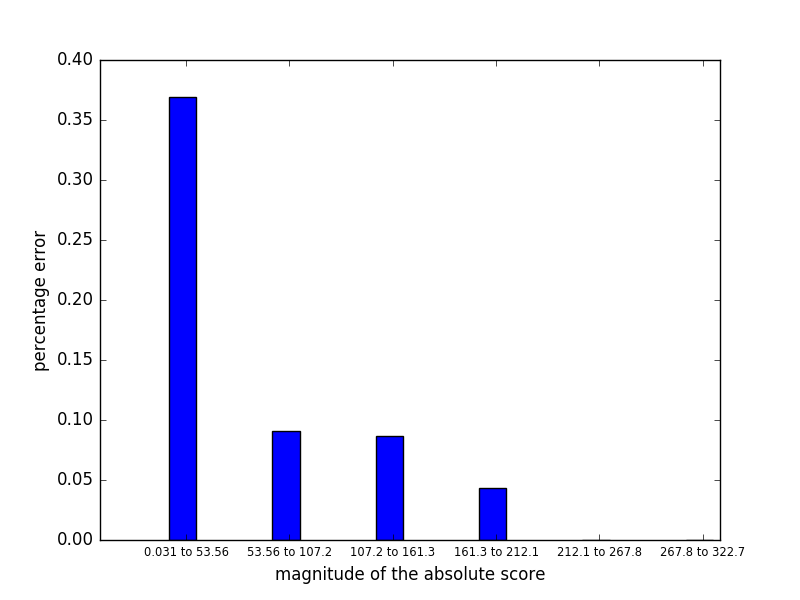
\includegraphics[width = 4in]{6_7.png}
\end{center}

From the plot we can see that, as the absolute magnitude increases, the percentage error decreases. For magnitude grater than  212.2 the algorithm gives perfect predictions.//

\pagebreak

\begin{problem}{6.8}
\end{problem}


\begin{minted}{python}
>>> pegasos_svm_sgd_2(X_train,y_train,lambda_ = lambda_opt,n_ite = 40,counter = True)
>>> 1.66666666667e-05
\end{minted} 

From the output, the non-differentiable case on occurs 1.666e-03 \% of the time. We can't skip the up date when $w^Tx_i = 0$. Since we initialized the weight to be 0, the first update will encounter the non-differentiable case. If we don't update the weight, the weight will be zero all the time. If we reinitialize the weight to be an non-zero vector, the skip might be feasible. 

\section{7 Error Analysis}

\begin{minted}{python}
def list_feature(X,w,n):
'''
show n heavily features of input x weight w

Args:
X: input data
w: weightes
n: number of features to be displayed

Returns: 4 by n array, r1:word, r2:number cotained in input, r3:weight, r4:contribution

'''
temp = Counter()
for i,j in w.items():
	temp[i] = abs(j*X[i])
res = np.zeros((4,n),dtype=object)
for k,i in enumerate(temp.most_common(n)):
	res[:,k] = i[0],X[i[0]],w[i[0]],abs(X[i[0]] *w[i[0]])
return res

>>> error_list = np.where(np.array(prediction) ==1)[0][:4]
>>> txt_error = X[error_list]
>>> res = []
>>> for i in txt_error:
   	 res.append(list_feature(i,w_opt,5))
    res = np.array(res)
>>> res
array([[['and', 'of', 'on', 'one', 'to'],
[22, 27, 8, 9, 20],
[-2.1177179750176767, -1.4637168356740076, 4.2042930386380801,
-3.6437206334863519, 1.4948597470713196],
[46.589795450388884, 39.520354563198204, 33.634344309104641,
32.793485701377165, 29.897194941426392]],

[['and', 'of', 'queen', 'on', 'to'],
[20, 16, 8, 4, 11],
[-2.1177179750176767, -1.4637168356740076, -2.6471474687721237,
4.2042930386380801, 1.4948597470713196],
[42.354359500353532, 23.419469370784121, 21.17717975017699,
16.817172154552321, 16.443457217784516]],

[['and', 'of', 'this', 'to', 'in'],
[25, 23, 14, 17, 16],
[-2.1177179750176767, -1.4637168356740076, 2.0242892408257243,
1.4948597470713196, -1.4948597470713221],
[52.94294937544192, 33.665487220502172, 28.340049371560141,
25.412615700212434, 23.917755953141153]],

[['only', 'and', 'on', 'to', 'in'],
[4, 13, 6, 15, 13],
[7.0382979757941211, -2.1177179750176767, 4.2042930386380801,
1.4948597470713196, -1.4948597470713221],
[28.153191903176484, 27.530333675229798, 25.225758231828479,
22.422896206069794, 19.433176711927189]]], dtype=object)
\end{minted}

From the above 4 examples that the model got wrong, we notice that the words which contribute the most are meaningless in the classification. Words such as 'and', 'of', 'on' are not explaining the text and thus are not good features even though the have large contributions. 

\section{8 Features}
\begin{sub}{8.1 Removing stop words}
\end{sub}

\begin{minted}{python}
def remover(x,sw):
	res = []
	for i in x:
		if i not in sw:
			res.append(i)
	return res

from nltk.corpus import stopwords
stopwords = stopwords.words("english")

X_train_new =np.array(map(lambda x:remover(x,sw = stopwords),X_train))

loss_list_3 = np.zeros(20)
for i,j in enumerate(try_list_2):
	w = pegasos_svm_sgd_2(X_train_new,y_train,lambda_= j,n_ite=20)
loss_list_3[i] = loss_0_1(X_test,y_test,w)

>>> loss_list_3
>>> array([ 0.2  ,  0.198,  0.2  ,  0.21 ,  0.18 ,  0.202,  0.206,  0.202,
0.206,  0.21 ,  0.2  ,  0.186,  0.194,  0.186,  0.198,  0.179,
0.192,  0.2  ,  0.202,  0.202])
\end{minted}

After removing the stop words in the text defined by nltk English Stopwords, and classify using svm, the best testing error was 0.179 which is slightly better than the previous model 

\pagebreak

\begin{sub}{8.2 Combine negations}
\end{sub}

\begin{minted}{python}
def remover_2(x,sw):
	res = []
	n = len(x)-1
	i=0
	negative = ['not',"aren't","isn't","doesn't","don't","didn't","hasn't"
			,"haven't","shoulden't","wouldn't","won't"]
	while i <= n:
		cur = x[i]
		if (cur not in sw) and (cur != 'not'):
			res.append(cur)
		elif cur == 'not' and i !=n:
			res.append(cur+'_'+x[i+1])
			i+=1
		i+=1
	return res
>>> X_train_2 = np.array(map(lambda x:remover_2(x,sw = stopwords),X_train))
>>> loss_list_4
array([ 0.208,  0.22 ,  0.186,  0.196,  0.222,  0.206,  0.2  ,  0.22 ,
0.21 ,  0.19 ,  0.198,  0.22 ,  0.2  ,  0.202,  0.208,  0.212,
0.184,  0.19 ,  0.206,  0.214])
\end{minted}

After combining the negation word with the word behind it and using it as a new features. The best testing error is 0.184
\end{document}



